% Created 2020-03-27 Fri 11:39
% Intended LaTeX compiler: pdflatex
\documentclass[presentation]{beamer}
\usepackage[utf8]{inputenc}
\usepackage[T1]{fontenc}
\usepackage{graphicx}
\usepackage{grffile}
\usepackage{longtable}
\usepackage{wrapfig}
\usepackage{rotating}
\usepackage[normalem]{ulem}
\usepackage{amsmath}
\usepackage{textcomp}
\usepackage{amssymb}
\usepackage{capt-of}
\usepackage{hyperref}
\usetheme{UoB}
\author{Mark Blyth}
\date{\textit{[2020-03-30 Mon]}}
\title{Discretisation-free CBC}
\hypersetup{
 pdfauthor={Mark Blyth},
 pdftitle={Discretisation-free CBC},
 pdfkeywords={},
 pdfsubject={},
 pdfcreator={Emacs 26.3 (Org mode 9.1.9)}, 
 pdflang={English}}
\begin{document}

\maketitle

\section{Background}
\label{sec:org74dc956}
\begin{frame}[label={sec:orgd33470a}]{Week's goal}
\begin{itemize}
\item Finish off redrafting paper
\item Start working towards an \emph{in-silico} CBC
\end{itemize}
\end{frame}

\begin{frame}[label={sec:org80e5494}]{Week's activities}
\begin{itemize}
\item Finished off redrafting paper
\item Started reading a paper for a single-cell model to test CBC on [1]
\begin{itemize}
\item Krasi's cubic Lienard model, but with a parameter fixed, and coupled to a slow subsystem
\item Capable of modelling almost all known bursting behaviours
\end{itemize}
\item Read some of Kuznetsov numerical bifurcation analysis
\item Started thinking about CBC
\begin{itemize}
\item This week's big idea: discretisation-free CBC
\end{itemize}
\end{itemize}

\vfill

[1] Saggio, Maria Luisa, et al. "Fast–slow bursters in the unfolding of a high codimension singularity and the ultra-slow transitions of classes." The Journal of Mathematical Neuroscience 7.1 (2017): 7.
\end{frame}

\section{Discretisation-free CBC}
\label{sec:org40faab0}
\begin{frame}[label={sec:org95abb1d}]{Continuation background: points}
\begin{itemize}
\item Continuation works in a predictor corrector scheme
\begin{itemize}
\item Predict the next point on the manifold from the local tangent vector
\item Correct it using a Newton iteration
\item An additional parameter appears -- the arclength parameter -- so require \emph{predictor \(\perp\) corrector} to ensure a well-posed problem
\end{itemize}
\item For equilibrium and equilibrium-bifurcation continuation, we have a finite-dimensional state
\begin{itemize}
\item Tangent vector is of the same dimensionality, and is therefore finite
\item Predictor-corrector scheme is of finite -- usually low -- dimensionality, and is therefore computationally tractable
\end{itemize}
\end{itemize}

For points (equilibria, equilibrium bifurcations) everything works nicely
\end{frame}

\begin{frame}[label={sec:org6412ecc}]{Continuation background: orbits}
\begin{itemize}
\item A periodic orbit is some function \(f(t,\lambda),~t\in[0,1]\)
\begin{itemize}
\item \(f\) exists in an infinite-dimensional Hilbert space
\end{itemize}
\item Continuation of \(f\) in \(\lambda\) requires a discretisation, to produce a finite-dimensional approximation that we can apply standard continuation methods on
\item There's a range of methods for discretisation
\begin{itemize}
\item Orthogonal collocation seeks a set of orthogonal polynomials that satisfy the model at a selection of meshpoints; high accuracy; requires a model
\item Fourier decomposition decomposes a periodic signal into its harmonic components; model-free (important for CBC); sensitive to noise; will be high-dimensional for spiking signals
\item Wavelets, frames, splines, \dots{}, yet to be developed!
\end{itemize}
\end{itemize}
\end{frame}

\begin{frame}[label={sec:org3a5838c}]{Issues with discretisation}
\begin{itemize}
\item Can't use collocation methods without a model
\item Spiking signals would need a lot of Fourier harmonics (quick-changing means lots of high-frequency energy); high dimensional continuation systems are hard
\item Noise would greatly impair Fourier discretisation; can't filter it off without losing the high-frequency components of the signal required for fast spiking
\item Wavelets, frames, splines haven't been developed yet (might also be noise-sensitive?)
\end{itemize}

Can we continue periodic orbits without discretisation?
\end{frame}

\begin{frame}[label={sec:orgd1565ea}]{Discretisation-free method: benefits and issues}
\begin{itemize}
\item By avoiding discretisation, we can deal with fast-changing signals easily
\item The learning step allows us to average out the noise, in a way that would be difficult using discretisation methods, meaning more numerical stability
\item Uses some machine learning -- a buzzword that seems to bring in citations\ldots{}
\item Fourier is a more natural discretisation choice for periodically excited systems
\begin{itemize}
\item If we can partition the control action into a controller and a periodic forcing term, it makes sense to do so
\item For neurons, where the stimulus and output are different, we can't do this partitioning, so we lose the benefits of Fourier
\end{itemize}
\end{itemize}
\end{frame}

\begin{frame}[label={sec:org510cf3b}]{Graphic representation}
\begin{center}
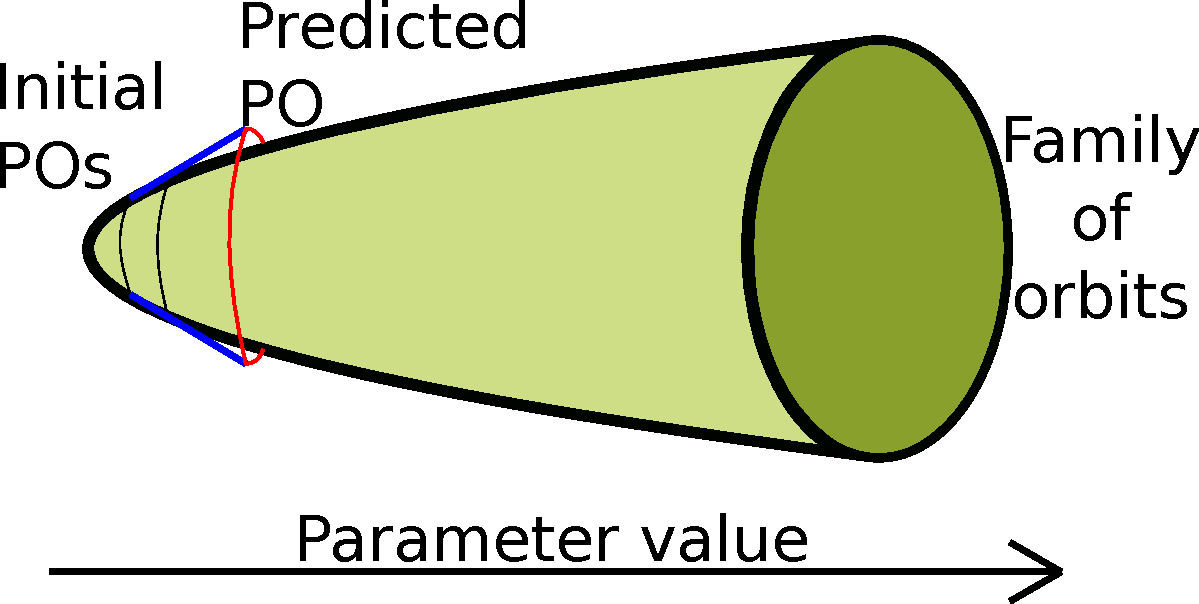
\includegraphics[width=.9\linewidth]{./po_family.pdf}
\end{center}
\end{frame}

\begin{frame}[label={sec:org333e646}]{Basic strategy}
\begin{itemize}
\item Learn a local model of the periodic orbit surface
\item Use that model to predict the next periodic orbit
\begin{itemize}
\item Learning and projecting forms the predictor step
\end{itemize}
\item Take the learned, predicted PO model as the control target
\item Iteratively update it, orthogonally to the forward-projection 
\begin{itemize}
\item This iterating forms the corrector step
\end{itemize}
\end{itemize}

No need to discretise the signal, as we fit a continuous model to the data and work from that instead.

\begin{itemize}
\item The zero problem is given by the noninvasive control requirement, rather than from a model
\item This means that we don't actually need to find a discretisation of the periodic orbit, unlike in model-based zero-problems
\end{itemize}
\end{frame}

\begin{frame}[label={sec:org41cdae7}]{A topology interlude}
\begin{itemize}
\item A homotopy \(H\) is a continuous deformation \(H:X \times [0,1] \to Y\) between two topological spaces \(X\) and \(Y\)
\item Consider a homotopy \(H\) between functions \(f_1\), \(f_2\), parameterised in some variable \(t\)
\begin{itemize}
\item \(H(f_1, 0) = f_1\)
\item \(H(f_1, 1) = f_2\)
\item Simple example: \(H = f_1 + t(f_2 - f_1)\)
\end{itemize}
\item \href{https://upload.wikimedia.org/wikipedia/commons/7/7e/HomotopySmall.gif}{Animation 1}
\item \href{https://en.wikipedia.org/wiki/Homotopy\#/media/File:Mug\_and\_Torus\_morph.gif}{Animation 2}
\end{itemize}

The overall goal is to learn a continuous homotopic transformation for the predictor/corrector, which can be applied to raw, undiscretised data
\end{frame}

\begin{frame}[label={sec:orged004a6}]{Mathematical representation}
\begin{itemize}
\item Use machine learning to find a homotopy between successive orbits \(f(t, \lambda_{i-1})\), \(f(t, \lambda_i)\)
\item Use this homotopy as a predictor for the next orbit
\item Apply an orthogonal correction step
\begin{itemize}
\item Prediction will be a smooth function estimating \(f(t, \lambda_1)\)
\item Find a corrector family of \(f\) orthogonal to the homotopic step
\item Each \(f\) in this family is a control target, one of which is a periodic orbit of the open-loop system
\item `Slide down' this family of periodic orbits, on to the corrected solution
\item `Sliding down' is done by iteratively updating the control target, much like in Barton et al.
\item By selecting new targets from the corrector family, we're maintaining the orthogonality constraint
\end{itemize}
\end{itemize}
\end{frame}

\begin{frame}[label={sec:org66ca0c3}]{Learning a homotopy}
\begin{enumerate}
\item Set \(\lambda = \lambda_0\)
\item Record data for a while
\item Use F\(_{\text{0}}\) estimator to partition data into periods
\item Reconstruct the state space (?)
\item Let \(t \in [0,1]\) measure how far through a period each reconstructed vector is
\item Learn a function \(f_0: [0,1] \to \mathbb{R}^n\), giving the (reconstructed) state at time \(t\)
\item Repeat this for \(\lambda = \lambda_1\), learning function \(f_1\)
\item Learn a homotopy \(H_1: \mathcal{H}\times [0,1] \to \mathcal{H}\), where \(f_i \in \mathcal{H}\)
\end{enumerate}
\end{frame}

\begin{frame}[label={sec:org93ebe57}]{The machine learning step}
\begin{itemize}
\item Gaussian processes are the ideal tool for learning \(f_i\), \(H_i\)
\begin{itemize}
\item Provide a nonparametric way of modelling arbitrary manifolds
\item Statistically rigorous
\end{itemize}
\item F\(_{\text{0}}\) estimation and state space reconstruction is much like that in my master's thesis
\item Might even be able to get away without the state space reconstruction, but intuitively it seems like everything would work better doing it
\end{itemize}
\end{frame}

\begin{frame}[label={sec:org555351f}]{Benefits and issues (again)}
\begin{itemize}
\item By avoiding discretisation, we can deal with exteedingly fast-changing signals easily
\item The learning step allows us to average out the noise, in a way that would be difficult using discretisation methods, meaning more numerical stability
\item Fourier is a more natural discretisation choice for periodically excited systems
\begin{itemize}
\item If we can partition the control action into a controller and a periodic forcing term, it makes sense to do so
\item For neurons, where the stimulus and output are different, we can't do this partitioning, so we lose the benefits of Fourier
\end{itemize}
\item Prediction step should be fairly straightforward
\item Correction step \emph{might} be straightforward, but has the potential to be more challenging
\end{itemize}
\end{frame}

\section{Next steps}
\label{sec:org855ef78}
\begin{frame}[label={sec:org84f33e4}]{Next steps}
\begin{itemize}
\item Finish readings (Kuznetsov numerical bifurcation analysis, neuron model paper)
\item Make any additional changes to the continuation paper
\item Further programming marking
\item Lab meeting Wednesday; make some slides for that
\begin{itemize}
\item Current plan: present everything I've written in the paper
\item Nb. I have managed to get Zoom to work, but can't use Skype for business
\end{itemize}
\item Try implementing Fourier CBC for a neuron
\item Adapt that for discretisation-free CBC
\end{itemize}
\end{frame}
\end{document}
